\chapter{Case studies}
To evaluate the effectiveness of the presented frameworks, we use three case studies. In each case
study, we benchmark the frameworks using the following steps:
\begin{enumerate}
    \item Describe the system of concern.
    \item Construct pDTMC models and formalize a reachability property.
    \item Select model true parameters and generate synthetic data.
    \item Apply the frameworks for both rational functions and simulation-based setups.
    \item Visualize the parameter synthesis and inference result.
    \item Measure runtime among different model sizes.
    \item Discussion on results.
\end{enumerate}
Three case studies include firstly a simple and standard case study \textit{IPv4 ZeroConfiguration
    Protocol}. The second case study comes from the experiments of the Department of Biology at the
University of Konstanz on the defensive behaviour of bee colonies\cite{hajnal2019data}. Third case
study is an epidemics model; it is introduced in order to show the expansion of the model
state-space as the system has more states to be encoded.\\
All experiments are conducted in the following system:
\begin{itemize}
    \item Intel Xeon W-2135 processor, 64GB RAM, OpenSUSE 15.2
    \item Python 3.8.8, StormPy 1.6.3, Storm stable, PRISM 4.6
\end{itemize}

%%%%%%%%%%%%%%%%%%%%%%%%%%%%%%%%%%%%%%%%%%%%%%%%%%%%%%%%%%%%%%%%%%%%%%%%%%%%%%%%%%%%%%%%%%%%%%%%%%%

\section{ZeroConfiguration Protocol}
\subsection{System description}
Zero-configuration protocol (\textit{zeroconf} for short) is a protocol used in IPv4 network to
allocate newly attached device an unique IP address without any intervention from network operators.
\begin{algorithm}[H]
    \caption{IPv4 Zeroconf procedure.}
    \label{alg:gen-sir-ctmc}
    \hspace*{\algorithmicindent} \textbf{Input:}
    \begin{itemize}
        \item $N$: number of probes.
    \end{itemize}
    \hspace*{\algorithmicindent} \textbf{Output:}
    \begin{itemize}
        \item An unused address
    \end{itemize}
    \begin{algorithmic}[1]
        \Procedure{Zeroconf}{}
        \State Select an address $ip$ randomly
        \State $i = 1$
        \While $i \leq N$
        \State Broadcast message asking if $ip$ is already in use.
        \If{Received reply that $ip$ is in use}
        \State Select an address $ip$ randomly
        \State Continue loop.
        \EndIf
        \If{timeout}
        \If{$i = N$}
        \State Return $ip$
        \EndIf
        \State $i \leftarrow i + 1$
        \State Continue loop.
        \EndIf
        \EndWhile
        \EndProcedure
    \end{algorithmic}
\end{algorithm}

\subsection{Model and properties}
We introduce two real parameters $(p, q) \in [0,1]\times[0,1]$.
\begin{itemize}
    \item $p$: probability of a message is loss (no reply and timed out).
    \item $q$: received a reply that $ip$ is in use.
\end{itemize}
By replace non-determinisms (timeout and address occupied) by probability distribution, we construct
the a pDTMC as a formalism of the Zeroconf protocol of $N$ probes.
\begin{figure}[H]
    \centering
    \begin{tikzpicture}[->, >=stealth', auto, semithick, node distance=2cm]
        \tikzstyle{every state}=[fill=white,draw=black,thick,text=black,scale=1]
        \node[state, initial]    (A)            {$S_0$};
        \node[state]    (B)[below of=A]         {};
        \node[state]    (I)[below of=B]         {$\text{OK}$};

        \node[state]    (C)[right of=A]         {$S_1$};
        \node[state]    (D)[right of=C]         {$S_2$};
        \node[state]    (E)[right of=D]         {$S_3$};
        \node[state]    (F)[right of=E]         {$S_4$};
        \node[state]    (G)[below of=F]         {};
        \node[state]    (H)[below of=G]         {$\text{Failed}$};

        \path
        (A)
        edge    node{$q$}       (C)
        edge    node{$1-q$}     (B)

        (B)
        edge    node{$1$}     (I)

        (I)
        edge [loop below] node{} (I)

        (C)
        edge    node{$p$}          (D)
        edge [bend left] node{$1-p$}        (A)

        (D)
        edge    node{$p$}          (E)
        edge  [bend left]  node{$1-p$}        (A)

        (E)
        edge    node{$p$}          (F)
        edge  [bend left]  node{$1-p$}        (A)

        (F)
        edge    node{$p$}          (G)
        edge [bend left]  node{$1-p$}        (A)

        (G)
        edge    node{$1$}          (H)

        (H)
        edge [loop below] node{} (G);

    \end{tikzpicture}
    \label{fig:zeroconf-4}
    \caption{IPv4 ZeroConf model, 4 probes}
\end{figure}

\begin{figure}[H]
    \centering
    \begin{tikzpicture}[->, >=stealth', auto, semithick, node distance=1.5cm]
        \tikzstyle{every state}=[fill=white,draw=black,thick,text=black,scale=0.75]
        \node[state, initial]    (A)            {$S_0$};
        \node[state]    (B)[below of=A]         {};
        \node[state]    (I)[below of=B]         {$\text{OK}$};

        \node[state]    (C)[right of=A]         {$S_1$};
        \node[state]    (D)[right of=C]         {$S_2$};
        \node[state]    (E)[right of=D]         {$S_3$};
        \node[state]    (F)[right of=E]         {$S_4$};
        \node[state]    (J)[right of=F]         {$S_5$};
        \node[state]    (K)[right of=J]         {$S_6$};
        \node[state]    (L)[right of=K]         {$S_7$};
        \node[state]    (M)[right of=L]         {$S_8$};
        \node[state]    (N)[right of=M]         {$S_9$};
        \node[state]    (O)[right of=N]         {$S_{10}$};

        \node[state]    (G)[below of=O]         {};
        \node[state]    (H)[below of=G]         {$\text{Failed}$};

        \path
        (A)
        edge    node{$q$}       (C)
        edge    node{$1-q$}     (B)

        (B)
        edge    node{$1$}     (I)

        (I)
        edge [loop below] node{} (I)

        (C)
        edge    node{$p$}          (D)
        edge [bend left] node{$1-p$}        (A)

        (D)
        edge    node{$p$}          (E)
        edge  [bend left]  node{$1-p$}        (A)

        (E)
        edge    node{$p$}          (F)
        edge  [bend left]  node{$1-p$}        (A)

        (F)
        edge    node{$p$}          (J)
        edge [bend left]  node{$1-p$}        (A)

        (J)
        edge    node{$p$}          (K)
        edge [bend left]  node{$1-p$}        (A)
        (K)
        edge    node{$p$}          (L)
        edge [bend left]  node{$1-p$}        (A)
        (L)
        edge    node{$p$}          (M)
        edge [bend left]  node{$1-p$}        (A)
        (M)
        edge    node{$p$}          (N)
        edge [bend left]  node{$1-p$}        (A)
        (N)
        edge    node{$p$}          (O)
        edge [bend left]  node{$1-p$}        (A)
        (O)
        edge    node{$p$}          (G)
        edge [bend left]  node{$1-p$}        (A)

        (G)
        edge    node{$1$}          (H)

        (H)
        edge [loop below] node{} (G);
    \end{tikzpicture}
    \label{fig:zeroconf-10}
    \caption{IPv4 ZeroConf model, 10 probes}
\end{figure}
We want to verify the following property:
\begin{align*}
    \text{Eventually, an IP is successfully allocated with at most $N$ probes with probability of at least 75 percents.}
\end{align*}
In PCTL formula
\begin{align*}
    P_{\geq 0.75} ( \texttt{true} \quad \mathsf{U}^{\leq N} \quad \texttt{"OK"} )
\end{align*}

\subsection{Evaluation}
\subsubsection{True parameters and synthetic data}
We use the following true parameter:
\begin{enumerate}
    \item Zeroconf 4 probes: $(p,q)=(0.10554747, 0.44965874)$
    \item Zeroconf 10 probes: $(p,q)=(0.19777902, 0.62182433)$
\end{enumerate}
Observation data $D_{obs}$ is from simulating the instantiated DTMC of true parameters $10000$ times.
\begin{figure}[H]
    \centering
    \begin{subfigure}{0.48\textwidth}
        \centering
        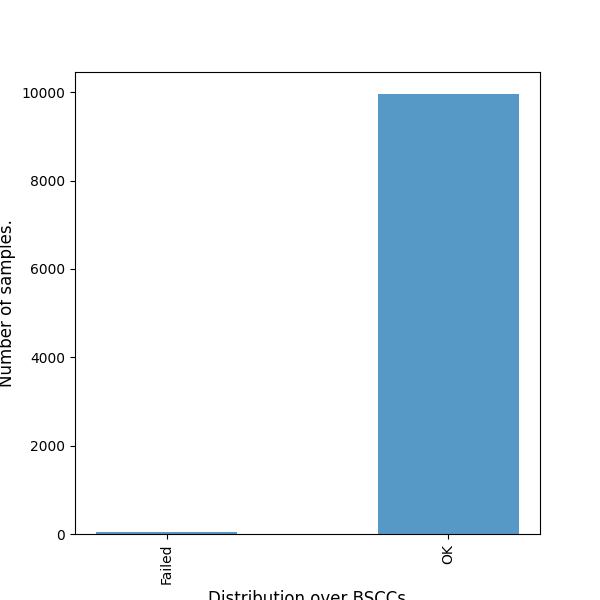
\includegraphics[width=\linewidth]{figures/zeroconf4_data.png}
        \caption{True parameters , $10000$ chain simulations.}
    \end{subfigure}
    \hfill
    \begin{subfigure}{0.48\textwidth}
        \centering
        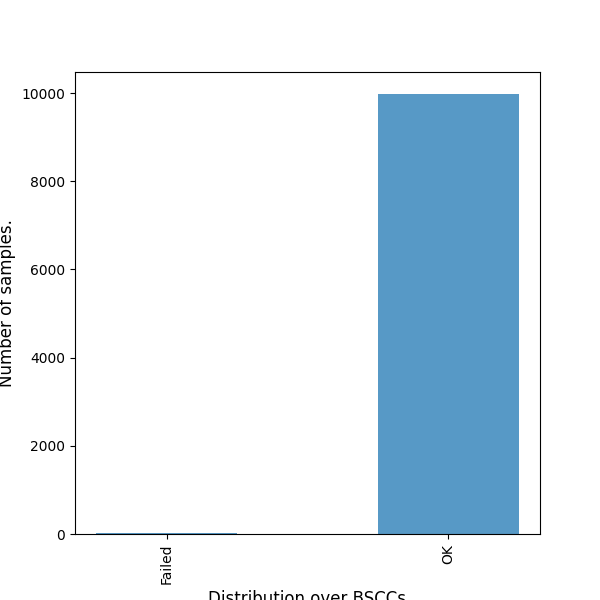
\includegraphics[width=\linewidth]{figures/zeroconf10_data.png}
        \caption{True parameters $(p,q)=(0.19777902, 0.62182433)$, $10000$ chain simulations.}
    \end{subfigure}
\end{figure}

\subsubsection{Parameter synthesis results}
Parameter synthesis for Zeroconf pDTMC of 4 probes.
\begin{table}[H]
    \begin{tabular}{|l|c|l|}
        \hline
        \multicolumn{1}{|c|}{\textbf{Zeroconf, 4 probes}} & \multicolumn{1}{l|}{\begin{tabular}[c]{@{}l@{}}Rational function\\ SMC\end{tabular}}                                   & \begin{tabular}[c]{@{}l@{}}Statistical model checking\\ ABC-SMC\end{tabular} \\ \hline
        True parameter                                    & \multicolumn{2}{c|}{(0.10554747, 0.44965874)}                                                                  \\ \hline
        Number of states                                  & \multicolumn{2}{c|}{9}                                                                                         \\ \hline
        Number of BSCCs                                   & \multicolumn{2}{c|}{2}                                                                                         \\ \hline
        Target property                                   & \multicolumn{2}{c|}{$P_{\geq 0.75} [!(i>2) \mathsf{U}^{\leq 4} (\texttt{"OK"})]$}                              \\ \hline
        Synthetic data                                    & \multicolumn{2}{c|}{$(41, 9959)$}                                                                              \\ \hline
        Inferred parameter point                          & \multicolumn{1}{l|}{$(0.18895572, 0.46055455)$}                                   & $(0.17646959, 0.35532204)$ \\ \hline
        L2 distance to true parameter                     & \multicolumn{1}{l|}{$0.08411690302113349$}                                        & $0.11802271422141228$      \\ \hline
        Run time (hh:mm:ss)                               & \multicolumn{1}{l|}{0:06:05.137928}                                               & 0:54:52.112848             \\ \hline
    \end{tabular}
    \caption{SIR(5,1,0) parameter estimation results.}
\end{table}

\begin{figure}[H]
    \centering
    \begin{subfigure}{0.48\textwidth}
        \centering
        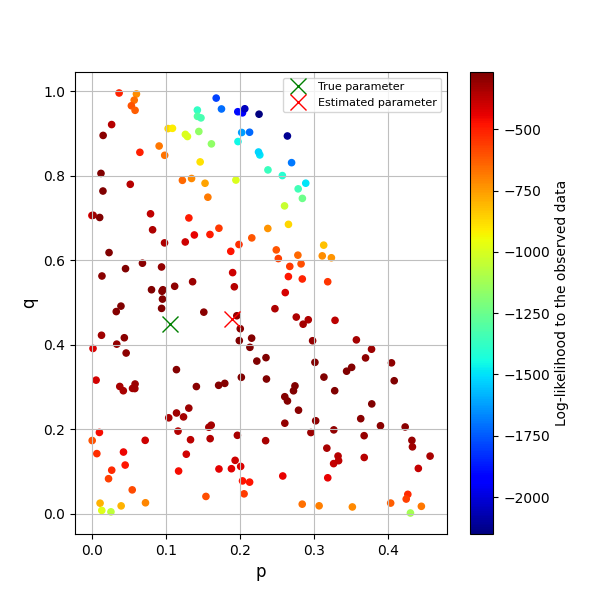
\includegraphics[width=\linewidth]{figures/zeroconf4_rf.png}
        \caption{Sampled particles using Rational Functions SMC}
    \end{subfigure}
    \hfill
    \begin{subfigure}{0.48\textwidth}
        \centering
        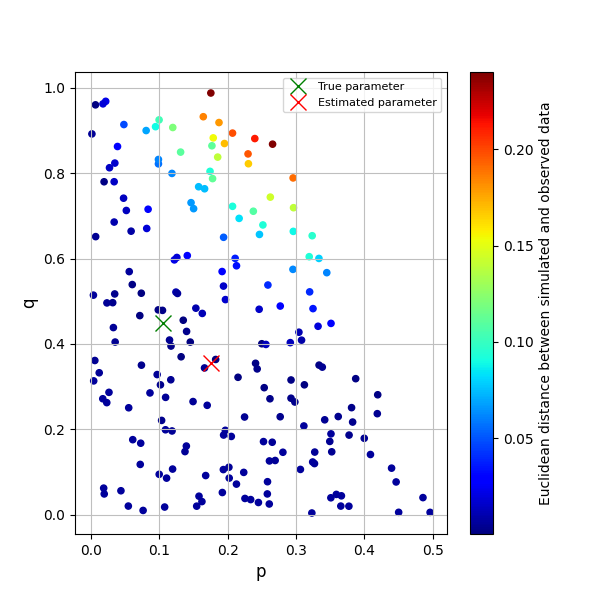
\includegraphics[width=\linewidth]{figures/zeroconf4_sim.png}
        \caption{Sampled particles using Statiscal Model Checking ABC-SMC}
    \end{subfigure}
\end{figure}

Parameter synthesis for Zeroconf pDTMC of 10 probes.
\begin{table}[H]
    \begin{tabular}{|l|c|l|}
        \hline
        \multicolumn{1}{|c|}{\textbf{Zeroconf, 4 probes}} & \multicolumn{1}{l|}{\begin{tabular}[c]{@{}l@{}}Rational function\\ SMC\end{tabular}}                                    & \begin{tabular}[c]{@{}l@{}}Statistical model checking\\ ABC-SMC\end{tabular} \\ \hline
        True parameter                                    & \multicolumn{2}{c|}{(0.19777902, 0.62182433)}                                                                   \\ \hline
        Number of states                                  & \multicolumn{2}{c|}{14}                                                                                         \\ \hline
        Number of BSCCs                                   & \multicolumn{2}{c|}{2}                                                                                          \\ \hline
        Target property                                   & \multicolumn{2}{c|}{$P_{\geq 0.75} [!(i>2) \mathsf{U}^{\leq 10} (\texttt{"OK"})]$}                              \\ \hline
        Synthetic data                                    & \multicolumn{2}{c|}{$(22, 9978)$}                                                                               \\ \hline
        Inferred parameter point                          & \multicolumn{1}{l|}{$(0.30180755, 0.45709018)$}                                    & $(0.37877446, 0.40586992)$ \\ \hline
        L2 distance to true parameter                     & \multicolumn{1}{l|}{$0.19483140118558434$}                                         & $0.2817723545992011$       \\ \hline
        Run time (hh:mm:ss)                               & \multicolumn{1}{l|}{0:09:29.760715}                                                & 0:37:56.507119             \\ \hline
    \end{tabular}
    \caption{SIR(5,1,0) parameter estimation results.}
\end{table}

\begin{figure}[H]
    \centering
    \begin{subfigure}{0.48\textwidth}
        \centering
        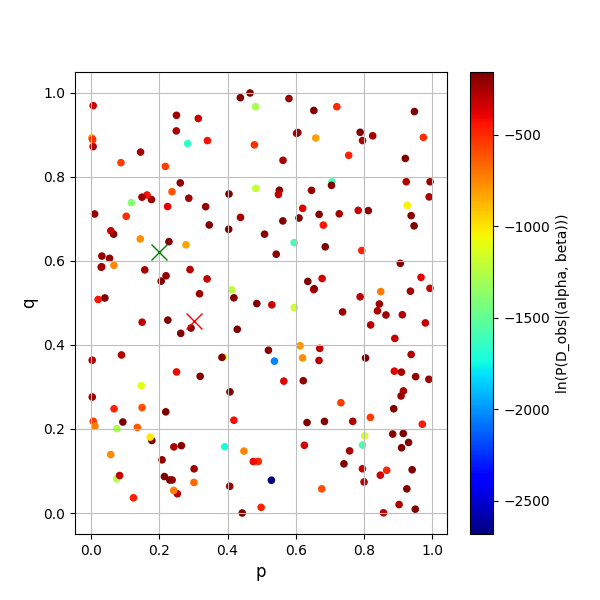
\includegraphics[width=\linewidth]{figures/zeroconf10_rf.png}
        \caption{Sampled particles using Rational Functions SMC}
    \end{subfigure}
    \hfill
    \begin{subfigure}{0.48\textwidth}
        \centering
        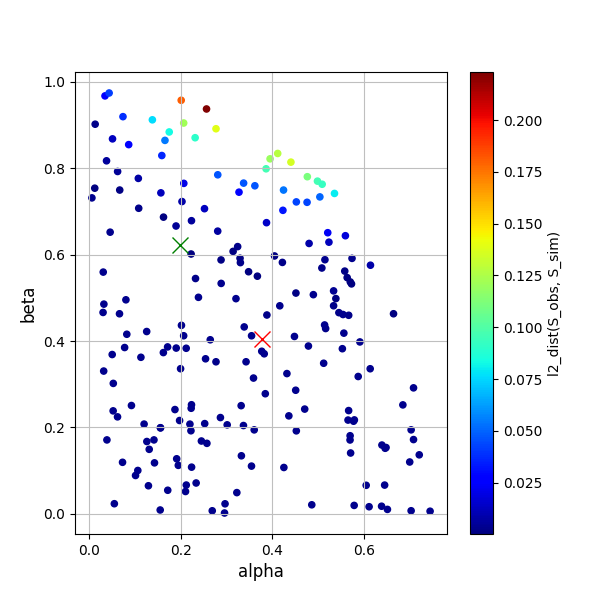
\includegraphics[width=\linewidth]{figures/zeroconf10_sim.png}
        \caption{Sampled particles using Statiscal Model Checking ABC-SMC}
    \end{subfigure}
\end{figure}

\subsection{Discussion}
For both model, rational function evaluation is faster than simulation. The simplicity of graphical
model gives simple rational function, so evaluating it is much faster than simulation, which
requires a lot of system calls to random generators. Both rational function evaluation and
simulation scheme are able to deliver a satisfying parameter estimation point. However, in Zeroconf
model of 10 probes, simulation has an advantage as the model transitions are simple topologically,
while rational function suffers from numerical error.

%%%%%%%%%%%%%%%%%%%%%%%%%%%%%%%%%%%%%%%%%%%%%%%%%%%%%%%%%%%%%%%%%%%%%%%%%%%%%%%%%%%%%%%%%%%%%%%%%%%
\section{Bees colony}
\subsection{System description}
We study the collective behavior of a bee colony. Each bee in a colony possibly stings after
observing a threat in the surrounding environment, and warn other bees by releasing a special
substance, pheromone. By sensing the pheromone released in the environment, other bees in the colony
may also sting. Assume that each bee in a colony decides its next action (to sting or not to sting)
based only on the current state of the environment, and the number of bees who sting or not sting
can be modeled as a Markov process. To reduce the complexity of the model, we make another
assumption that the states of the bees colony are observed after uniform time duration, hence the
model is of discrete-time. However, since stinging leads to the termination of an individual bee, it
reduces the total defense capability as well.

\subsection{Model and properties}
With parametric Discrete-time Markov chain as the model, we study how the actions of a single bee
change with regarding to the colony size of and pheromone amount.There are 3 assumptions on the
system:
\begin{enumerate}
    \item Each bee release an unit amount of pheromone immediately after stinging.
    \item A bee dies after stinging and releasing pheromone. In the other words, no bee can sting
          more than once.
    \item Stinging behaviour only depends on the concentration of pheromone in the environment.
\end{enumerate}
Under these assumption, a bee colony can be viewed as a set of agents (bees) interact with each
other in a closed environment with the appearance of a factor \textit{pheromone}. Afterward, the
agent has probability to commit an action, namely \textit{sting}. The agent is eliminated from
environment after stinging. Assume that we have a colony of $n$ bees initially. As aforementioned,
an individual bee is terminated after it stings. Thus, at the end of experiment, the number of bees
is $n'\in\{0,1,\ldots,n\}$. We model the bee colony with a DTMC $\mathcal{M}=(S,\mathbf{P},
    S_{init}, AP,L)$, such that
\begin{itemize}
    \item $|S_{init}|=1$
    \item There exists $n+1$ tSCCs which encode the population at the end of the experiment.
\end{itemize}
Semantics of \textit{semi-synchronous} Markov population models for bees colony are developed by
\cite{hajnal2019data}.
\begin{itemize}
    \item \textit{Synchronous model}:
\end{itemize}
In \textit{semisynchronous model}, we assume that the behaviour is initally synchronous. From all
succeeding states from initial states, the updates are of asynchronous semantics.
\begin{example}{Semisynchronous model of 3 bees.}
    We model a colony of 3 bees using semisynchronous semantics. In the following DTMC model, each
    individual bee is encode by an integer represents its state
    \begin{itemize}
        \item 0: bee never stings.
        \item 1: bee stings and dies.
        \item 2: bee does not sting in 2 consecutive observations.
    \end{itemize}
    Let $p, q_1, q_2$ represent the probabilities that a bee stings without any stimulation and a
    bee stings at 1 and 2 attemps, respectively. We then construct the following pDTMC
    \begin{figure}[H]
        \centering
        \begin{tikzpicture}[->, >=stealth', auto, semithick, node distance=4cm]
            \tikzstyle{every state}=[fill=white,draw=black,thick,text=black,scale=1]
            \node[state,initial]    (A)                     {init};
            \node[state]            (B)[right of=A]         {$2, 2, 1 $};
            \node[state]            (C)[above of=B]         {$0, 0, 0$};
            \node[state]            (D)[below of=B]         {$2, 1, 1$};
            \node[state,accepting]  (E)[below of=D]         {$1, 1, 1$};
            \node[state]            (F)[right of=B]         {$0, 2, 1$};
            \node[state,accepting]  (G)[right of=D]         {$0, 1, 1$};
            \node[state,accepting]  (H)[right of=F]         {$0, 0, 1$};
            \path
            (A)
            edge    node{$3p(1-p)^2$}      (B)
            edge    node{$(1-p)^3$}        (C)
            edge    node{$3p(1-p)^2$}      (D)
            edge    node{$p^3$}            (E)
            (B)
            edge    node{$1-q_1$}            (F)
            edge    node{$q_1$}              (D)

            (D)
            edge    node{$1-q_2$}          (G)
            edge    node{$q_2$}              (E)
            (F)
            edge    node{$q_1$}              (G)
            edge    node{$1 - q_1$}          (H);
        \end{tikzpicture}
        \caption{Semisynchronous model of 3 bees, 3 parameters $p, q_1, q_2$)}
    \end{figure}
\end{example}
We verify the following property:
\begin{align*}
    \text{With probability of at least 25 percents, at least a half of bees population survives.}
\end{align*}
In PCTL formula
\begin{align*}
    P_{\geq 0.25} ( \texttt{true} \quad \mathsf{U} \quad \texttt{"|Survived| > 0.5N"} )
\end{align*}

\subsection{Evaluation}
\subsubsection{True parameters and synthetic data}
We use the following true parameter:
\begin{table}[]
    \begin{tabular}{|l|l|l|}
        \hline
                        & Semisynchronous model, 3 bees        & Semisynchronous model, 5 bees       \\ \hline
        Number of BSCCs & 4                                    & 6                                   \\ \hline
        True parameter  & (0.66562362, 0.83040077, 0.83977757) & \begin{tabular}[c]{@{}l@{}}(0.2783698,  0.30599383, 0.4897924,\\   0.73725233, 0.76658066)\end{tabular}          \\ \hline
        Synthetic data  & (344,   54, 1390, 8212)              & (1940,   11,  216, 2682, 4200, 951) \\ \hline
    \end{tabular}
\end{table}
Observation data $D_{obs}$ is from simulating the instantiated DTMC of true parameters $10000$ times.
\begin{figure}[H]
    \centering
    \begin{subfigure}{0.48\textwidth}
        \centering
        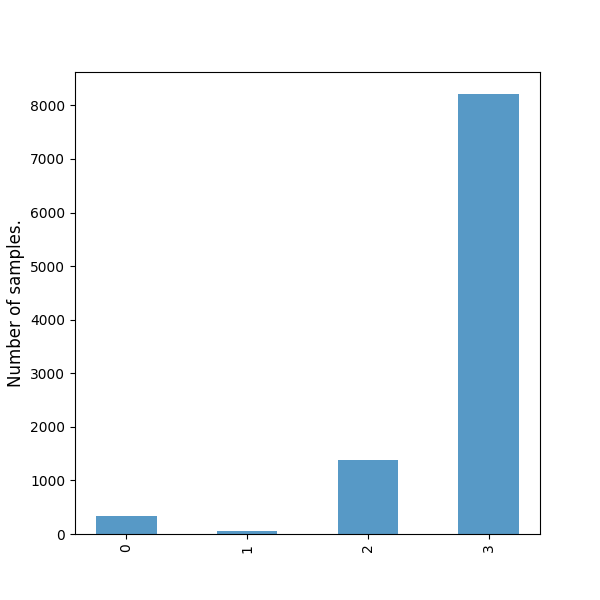
\includegraphics[width=\linewidth]{figures/bee_3_data.png}
        \caption{True parameters , $10000$ chain simulations.}
    \end{subfigure}
    \hfill
    \begin{subfigure}{0.48\textwidth}
        \centering
        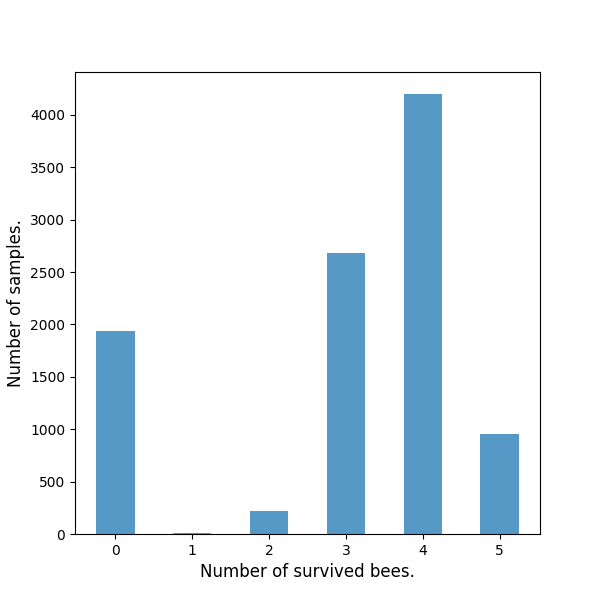
\includegraphics[width=\linewidth]{figures/bee_5_data.png}
        \caption{True parameters, $10000$ chain simulations.}
    \end{subfigure}
\end{figure}

\subsubsection{Parameter synthesis results}
Parameter synthesis for semisynchronous model of 3 bees.
\begin{table}[H]
    \begin{tabular}{|l|l|l|}
        \hline
        {\color[HTML]{232627} Semisynchronous model, 3 bees} & \begin{tabular}[c]{@{}l@{}}SMC with\\ rational function\end{tabular}                                & \begin{tabular}[c]{@{}l@{}}ABC-SMC with\\ statistical model checking\end{tabular} \\ \hline
        True parameter                                       & \multicolumn{2}{c|}{(0.66562362, 0.83040077, 0.83977757)}                              \\ \hline
        Estimated parameter                                  & \begin{tabular}[c]{@{}c@{}}(0.67138814, 0.57502566,\\   0.52550228)\end{tabular}                                & \begin{tabular}[c]{@{}c@{}}(0.81165139, 0.62107331,\\   0.5441299)\end{tabular} \\ \hline
        L2 distance                                          & 0.40499214733462613                                       & 0.3905759806675119         \\ \hline
        Time elapsed                                         & 0:05:55.157159                                            & 1:08:47.830380             \\ \hline
    \end{tabular}
\end{table}


Parameter synthesis for semisynchronous model of 5 bees.
\begin{table}[H]
    \begin{tabular}{|l|l|l|}
        \hline
        {\color[HTML]{232627} Semisynchronous model, 5 bees} & \begin{tabular}[c]{@{}l@{}}SMC with\\ rational function\end{tabular}                      & \begin{tabular}[c]{@{}l@{}}ABC-SMC with\\ statistical model checking\end{tabular} \\ \hline
        True parameter                                       & \multicolumn{2}{c|}{\begin{tabular}[c]{@{}c@{}}(0.2783698,  0.30599383, 0.4897924,\\   0.73725233, 0.76658066)\end{tabular}}                              \\ \hline
        Estimated parameter                                  & \begin{tabular}[c]{@{}l@{}}(0.57656519, 0.58972387,\\  0.49033413, 0.55439667,\\  0.52443301)\end{tabular}                      & \begin{tabular}[c]{@{}l@{}}(0.36121979, 0.31600669,\\  0.5456908, 0.64396223,\\  0.59120587)\end{tabular} \\ \hline
        L2 distance                                          & 0.511366013681474                               & 0.22259463218787823        \\ \hline
        Time elapsed                                         & 0:29:31.224466                                  & 5:52:05.296708             \\ \hline
    \end{tabular}
\end{table}

\subsection{Discussion}
The case study with bee colony we observed that both simulation-based framework and rational
function based framework deliver estimations which are close to the true parameter. However, the
simulation-based framework is much more expensive computationally. In the experiment with 5 bees, it
is shown that the simulation-based framework obtain better estimation to the true parameter.
However, the result is not conclusive since the algorithm is randomized, and more experiments must
be conducted to have enough data to conclude the effectiveness of two frameworks.

%%%%%%%%%%%%%%%%%%%%%%%%%%%%%%%%%%%%%%%%%%%%%%%%%%%%%%%%%%%%%%%%%%%%%%%%%%%%%%%%%%%%%%%%%%%%%%%%%%%
\section{SIR model}
\subsection{System}
\textit{SIR} model  is a population model, which is widely used in modeling epidemics. In a
\text{SIR} model, each individual is of one among three types:
\begin{itemize}
    \item \textit{Susceptible (S)}
    \item \textit{Infected (S)}
    \item \textit{Recovered (S)}
\end{itemize}
SIR system is a stochastic system modeled by reactions between S, I and R. In this thesis we use
only 2 reactions.
\begin{align*}
    R_1: & S + I \xrightarrow{\alpha} 2I \\
    R_2: & I     \xrightarrow{\beta} R
\end{align*}

\begin{algorithm}[H]
    \caption{Generate SIR CTMC from reactions.}
    \label{alg:gen-sir-ctmc}
    \hspace*{\algorithmicindent} \textbf{Input:}
    \begin{itemize}
        \item $(S_0, I_0, R_0)$: initial population.
        \item Reactions of rate $\alpha,\beta$
              \begin{align*}
                  R_1: & S + I \xrightarrow{\alpha} 2I \\
                  R_2: & I     \xrightarrow{\beta} R
              \end{align*}
    \end{itemize}
    \hspace*{\algorithmicindent} \textbf{Output:}
    \begin{itemize}
        \item CTMC $\mathcal{C}$
    \end{itemize}
    \begin{algorithmic}[1]
        \Procedure{Explore}{$s$,$i$,$r$}
        \If{$i = 0$}
        \State Mark $(s,i,r)$ as a BSCC.
        \State Return
        \EndIf
        \If{$(s>0) \wedge (i>0)$}
        \If{State $(s-1, i+1, r)$ already visited}
        \State Return
        \EndIf
        \State Add $(s-1, i+1, r)$ to state space
        \State Explore($s-1$, $i+1$,$r$)
        \EndIf
        \If{$(i>0)$}
        \If{State $(s, i-1, r+1)$ already visited}
        \State Return
        \EndIf
        \State Add $(s, i-1, r+1)$ to state space
        \State Explore($s$, $i-1$,$r+1$)
        \EndIf
        \EndProcedure
        \Procedure{Sir-Explore-Statespace}{$s_0,i_0,r_0$}
        \State Sir-Explore-Statespace$(s_0,i_0,r_0)$
        \EndProcedure
    \end{algorithmic}
\end{algorithm}

\subsection{Model and properties}
\begin{theorem}{Acyclicity}
    A CTMC $\mathcal{C}$ constructed by Algorithm \ref{alg:gen-sir-ctmc} using reactions
    $R_1, R_2$ is acyclic.
\end{theorem}
\textbf{Proof}: For any arbitrary transition in $\mathcal{C}$
\begin{enumerate}
    \item $|S|$ is monotonically decreasing, as there exists no reaction which produces $S$.
    \item $|R|$ is monotonically increasing, as there exists no reaction which consumes $R$.
    \item If $P((s,i,r), (s',i',r'))\neq 0$, then $i \neq i'$. That is because all reactions change $i$.
\end{enumerate}
As $|S| + |I| + |R| = S_0 + I_0 + R_0$ and $S_0,R_0,I_0$ are constants, if there exists a path fragment
\begin{align*}
    (s^t,i^t,r^t)\rightarrow \quad \ldots \quad \rightarrow(s^{t+k},i^{t+k},r^{t+k})
\end{align*}
such that $(s^t,i^t,r^t) = (s^{t+k},i^{t+k},r^{t+k})$ then $k=0$, because all reactions change $i$
(if $P((s,i,r), (s',i',r'))\neq 0$, then $i \neq i'$). \QED
\begin{corollary}
    A CTMC constructed by Algorithm \ref{alg:gen-sir-ctmc} using reactions $R_1, R_2$ has BSCCs
    and the BSCCs are trivial.
\end{corollary}

\begin{example}
    Example of an SIR CTMC model with initial population $(S_0, I_0, R_0) = (3,1,0)$
    \begin{figure}[H]
        \centering
        \begin{tikzpicture}[->, >=stealth', auto, semithick, node distance=3cm]
            \tikzstyle{every state}=[fill=white,draw=black,thick,text=black]
            \node[state]    (Init)                      {$(3,1,0)$};
            \node[state]    (S_301)[below of=Init]      {$(3,0,1)$};
            \node[state]    (S_220)[right of=Init]      {$(2,2,0)$};
            \node[state]    (S_211)[below of=S_220]     {$(2,1,1)$};
            \node[state]    (S_202)[below of=S_211]     {$(2,0,2)$};
            \node[state]    (S_130)[right of=S_220]     {$(1,3,0)$};
            \node[state]    (S_121)[below of=S_130]     {$(1,2,1)$};
            \node[state]    (S_112)[below of=S_121]     {$(1,1,2)$};
            \node[state]    (S_103)[below of=S_112]     {$(1,0,3)$};
            \node[state]    (S_040)[right of=S_130]     {$(0,4,0)$};
            \node[state]    (S_031)[below of=S_040]     {$(0,3,1)$};
            \node[state]    (S_022)[below of=S_031]     {$(0,2,2)$};
            \node[state]    (S_013)[below of=S_022]     {$(0,1,3)$};
            \node[state]    (S_004)[below of=S_013]     {$(0,0,4)$};
            \path
            (Init)
            edge node{$\beta$} (S_301)
            edge node{$3\alpha$} (S_220)

            (S_220)
            edge node{$2\alpha$} (S_130)
            edge node{$\beta$} (S_211)

            (S_130)
            edge node{$\alpha$} (S_040)
            edge node{$3\beta$} (S_121)

            (S_040)
            edge node{$4\beta$} (S_031)

            (S_031)
            edge node{$3\beta$} (S_022)

            (S_022)
            edge node{$2\beta$} (S_013)

            (S_013)
            edge node{$\beta$} (S_004)

            (S_121)
            edge node{$\alpha$} (S_031)
            edge node{$\beta$} (S_112)

            (S_112)
            edge node{$\alpha$} (S_022)
            edge node{$\beta$} (S_103)

            (S_211)
            edge node{$2\alpha$} (S_121)
            edge node{$\beta$} (S_202)

            (S_301)
            edge [in=240,out=300,loop]  ()

            (S_202)
            edge [in=240,out=300,loop]  ()

            (S_103)
            edge [in=240,out=300,loop]  ()

            (S_004)
            edge [in=240,out=300,loop]  ();

        \end{tikzpicture}
        \caption{$SIR(3,1,0)$ CTMC model with parameters$(\alpha, \beta)$}
    \end{figure}
\end{example}

\begin{example}
    Uniformize the chain with uniformization rate $(3\alpha + 4\beta)$, we derive the following uniformized DTMC:
    \begin{figure}[H]
        \centering
        \begin{tikzpicture}[->, >=stealth', auto, semithick, node distance=3.5cm]
            \tikzstyle{every state}=[fill=white,draw=black,thick,text=black]
            \node[state]    (Init)                      {$(3,1,0)$};
            \node[state]    (S_301)[below of=Init]      {$(3,0,1)$};
            \node[state]    (S_220)[right of=Init]      {$(2,2,0)$};
            \node[state]    (S_211)[below of=S_220]     {$(2,1,1)$};
            \node[state]    (S_202)[below of=S_211]     {$(2,0,2)$};
            \node[state]    (S_130)[right of=S_220]     {$(1,3,0)$};
            \node[state]    (S_121)[below of=S_130]     {$(1,2,1)$};
            \node[state]    (S_112)[below of=S_121]     {$(1,1,2)$};
            \node[state]    (S_103)[below of=S_112]     {$(1,0,3)$};
            \node[state]    (S_040)[right of=S_130]     {$(0,4,0)$};
            \node[state]    (S_031)[below of=S_040]     {$(0,3,1)$};
            \node[state]    (S_022)[below of=S_031]     {$(0,2,2)$};
            \node[state]    (S_013)[below of=S_022]     {$(0,1,3)$};
            \node[state]    (S_004)[below of=S_013]     {$(0,0,4)$};
            \path[->, every loop/.style={looseness=3}]
            (Init)
            edge node{$\frac{\beta}{3\alpha + 3\beta}$}   (S_301)
            edge node{$\frac{3\alpha}{3\alpha + 3\beta}$} (S_220)
            edge[in=150,out=105,loop] node[above]{$\frac{3\beta}{3\alpha + 3\beta}$} ()

            (S_220)
            edge node{$\frac{2\alpha}{3\alpha + 3\beta}$} (S_130)
            edge node{$\frac{\beta}{3\alpha + 3\beta}$} (S_211)
            edge[in=150,out=105,loop] node[above]{$\frac{\alpha+3\beta}{3\alpha + 3\beta}$} ()

            (S_130)
            edge node{$\frac{\alpha}{3\alpha + 3\beta}$} (S_040)
            edge node{$\frac{3\beta}{3\alpha + 3\beta}$} (S_121)
            edge[in=150,out=105,loop] node[above]{$\frac{2\alpha+\beta}{3\alpha + 3\beta}$} ()

            (S_040)
            edge node{$\frac{4\beta}{3\alpha + 3\beta}$} (S_031)
            edge[in=150,out=105,loop] node[above]{$\frac{3\alpha}{3\alpha + 3\beta}$} ()

            (S_031)
            edge node{$\frac{3\beta}{3\alpha + 3\beta}$} (S_022)
            edge[in=150,out=105,loop] node[above]{$\frac{3\alpha+\beta}{3\alpha + 3\beta}$} ()

            (S_022)
            edge node{$\frac{2\beta}{3\alpha + 3\beta}$} (S_013)
            edge[in=150,out=105,loop] node[above]{$\frac{3\alpha + 2\beta}{3\alpha + 3\beta}$} ()

            (S_013)
            edge node{$\frac{\beta}{3\alpha + 3\beta}$} (S_004)
            edge[in=150,out=105,loop] node[above]{$\frac{3\alpha + 3\beta}{3\alpha + 3\beta}$} ()

            (S_121)
            edge node{$\frac{\alpha}{3\alpha + 3\beta}$} (S_031)
            edge node{$\frac{\beta}{3\alpha + 3\beta}$} (S_112)
            edge[in=150,out=105,loop] node[above]{$\frac{2\alpha + 3\beta}{3\alpha + 3\beta}$} ()

            (S_112)
            edge node{$\frac{\alpha}{3\alpha + 3\beta}$} (S_022)
            edge node{$\frac{\beta}{3\alpha + 3\beta}$} (S_103)
            edge[in=150,out=105,loop] node[above]{$\frac{2\alpha+3\beta}{3\alpha + 3\beta}$} ()

            (S_211)
            edge node{$\frac{2\alpha}{3\alpha + 3\beta}$} (S_121)
            edge node{$\frac{\beta}{3\alpha + 3\beta}$} (S_202)
            edge[in=150,out=105,loop] node[above]{$\frac{\alpha+3\beta}{3\alpha + 3\beta}$} ()

            (S_301)
            edge [in=240,out=300,loop]  ()

            (S_202)
            edge [in=240,out=300,loop]  ()

            (S_103)
            edge [in=240,out=300,loop]  ()

            (S_004)
            edge [in=240,out=300,loop]  ();

        \end{tikzpicture}
        \caption{$SIR(3,1,0)$ Uniformized DTMC model with parameters$(\alpha, \beta)$ and uniformization rate $(3\alpha + 4\beta)$}
    \end{figure}
\end{example}
We check the following property: "With probability of at least 25 percents, the number of infected individuals does not exceed half of the population until the system is stabilized."
In PCTL formula:
\begin{align*}
    P_{\geq 0.25} ( !(i > (S_0 + i_0 + R_0)/2) \quad \mathsf{U} \quad (i = 0) )
\end{align*}


\subsection{Evaluation}
\subsubsection{True parameters and synthetic data}
\subsubsection{Parameter synthesis result}
We evaluate simulation-based and rational function based frameworks on different size of initial population.
\begin{figure}[H]
    \centering
    \begin{subfigure}{0.3\textwidth}
        \centering
        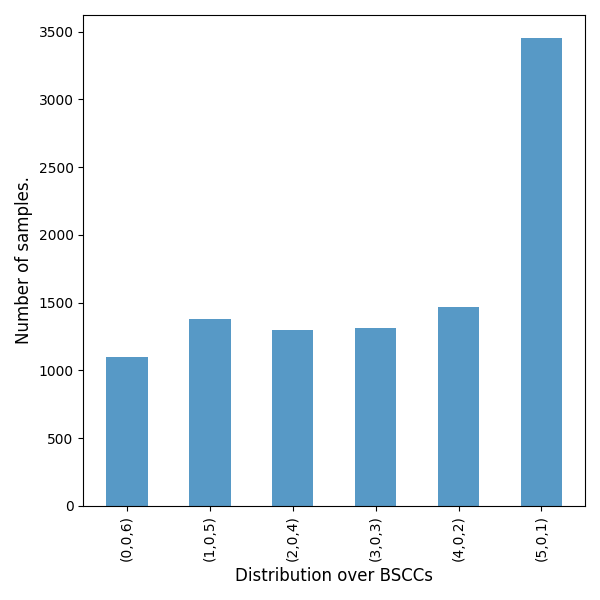
\includegraphics[width=\linewidth]{figures/sir510_data.png}
        \caption{SIR(5,1,0) synthetic data}
    \end{subfigure}
    \hfill
    \begin{subfigure}{0.3\textwidth}
        \centering
        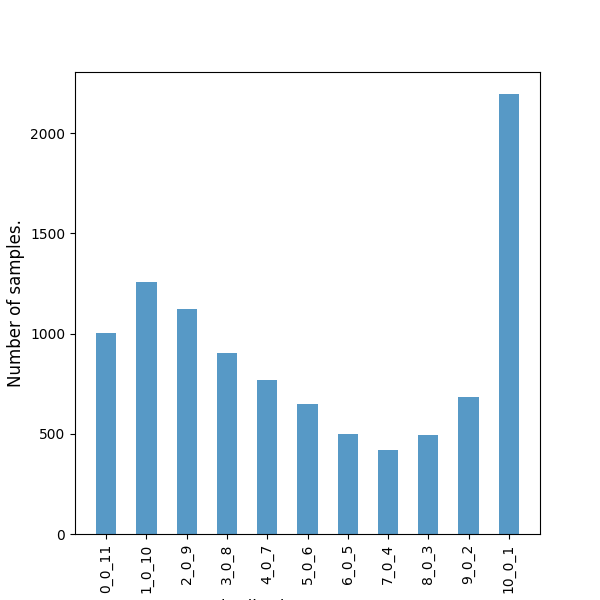
\includegraphics[width=\linewidth]{figures/sir1010_data.png}
        \caption{SIR(5,1,0) synthetic data}
    \end{subfigure}
    \hfill
    \begin{subfigure}{0.3\textwidth}
        \centering
        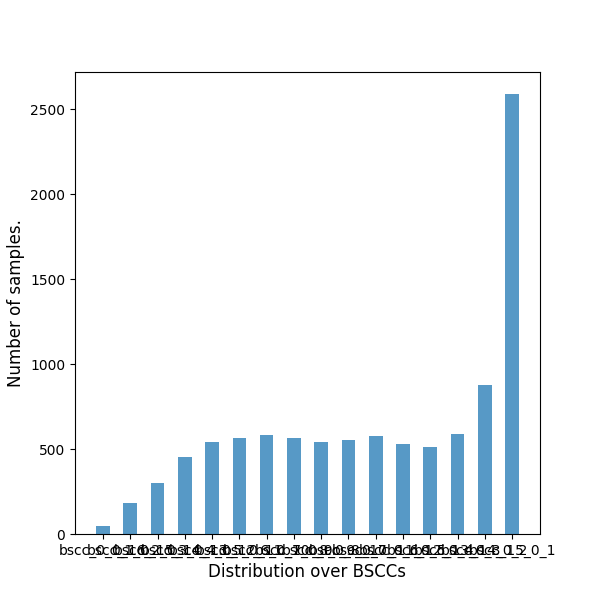
\includegraphics[width=\linewidth]{figures/sir1510_data.png}
        \caption{SIR(5,1,0) synthetic data}
    \end{subfigure}
    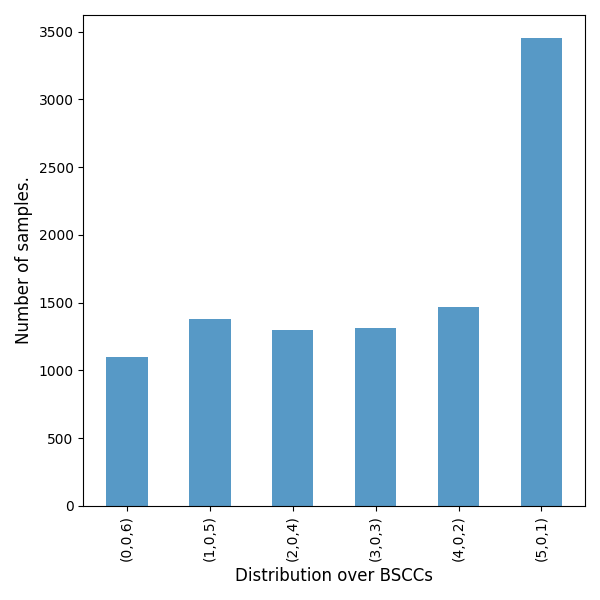
\includegraphics[width=0.45\linewidth]{figures/sir510_data.png}
    \caption{Synthetic data $D_{obs}$ using selected true parameter.}
\end{figure}

\begin{table}[H]
    \begin{tabular}{|l|c|l|}
        \hline
        \multicolumn{1}{|c|}{\textbf{SIR(5,1,0)}} & \multicolumn{1}{l|}{\begin{tabular}[c]{@{}l@{}}Rational function\\ SMC\end{tabular}}            & \begin{tabular}[c]{@{}l@{}}Statistical model checking\\ ABC-SMC\end{tabular} \\ \hline
        True parameter                            & \multicolumn{2}{c|}{(0.03405521, 0.08773454)}                                           \\ \hline
        Number of states                          & \multicolumn{2}{c|}{27}                                                                 \\ \hline
        Number of BSCCs                           & \multicolumn{2}{c|}{6}                                                                  \\ \hline
        Target property                           & \multicolumn{2}{c|}{$P_{\geq 0.25} [!(i>3) U^{<6} (i=0)]$}                              \\ \hline
        Synthetic data                            & \multicolumn{2}{c|}{(1098, 1377, 1296, 1312, 1466, 3451)}                               \\ \hline
        Inferred parameter point                  & \multicolumn{1}{l|}{(0.02547391, 0.0676129)}               & (0.02307652, 0.06481155)   \\ \hline
        L2 distance to true parameter             & \multicolumn{1}{l|}{0.021875082353604854}                  & 0.02011985105552338        \\ \hline
        Run time (hh:mm:ss)                       & \multicolumn{1}{l|}{0:19:34.397596}                        & 3:51:36.893424             \\ \hline
    \end{tabular}
    \caption{SIR(5,1,0) parameter estimation results.}
\end{table}

\begin{figure}[H]
    \centering
    \begin{subfigure}{0.48\textwidth}
        \centering
        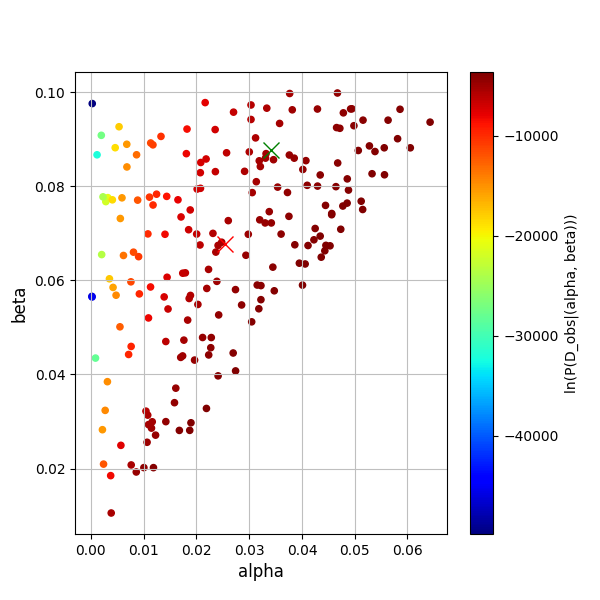
\includegraphics[width=\linewidth]{figures/sir510_rfsmc.png}
        \caption{Sampled particles using Rational Functions SMC}
    \end{subfigure}
    \hfill
    \begin{subfigure}{0.48\textwidth}
        \centering
        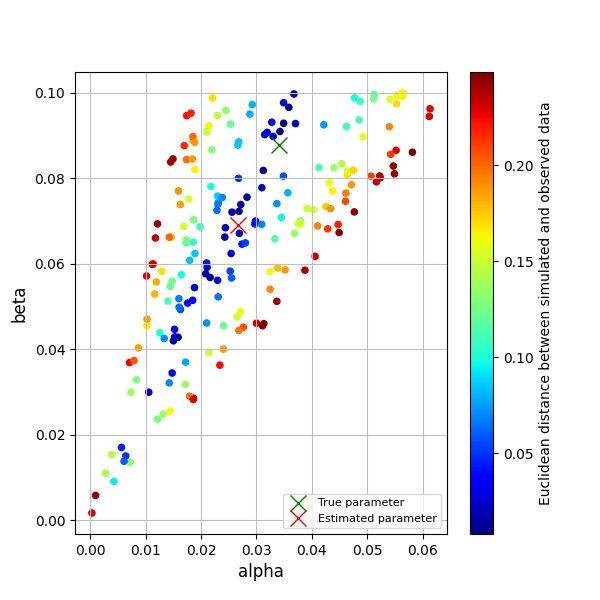
\includegraphics[width=\linewidth]{figures/sir510_abcsmc.png}
        \caption{Sampled particles using Statiscal Model Checking ABC-SMC}
    \end{subfigure}
    \caption{SIR(5,1,0) parameter synthesis results.}
\end{figure}

In the experiment with $SIR(5,1,0)$ model we can see that rational-function based method and simulation based method deliver results without significantly difference.

\begin{table}[H]
    \begin{tabular}{|l|c|l|}
        \hline
        \multicolumn{1}{|c|}{\textbf{SIR(10,1,0)}} & \multicolumn{1}{l|}{\begin{tabular}[c]{@{}l@{}}Rational function\\ SMC\end{tabular}}                                        & \begin{tabular}[c]{@{}l@{}}Statistical model checking\\ ABC-SMC\end{tabular} \\ \hline
        True parameter                             & \multicolumn{2}{c|}{(0.02549012, 0.0692981)}                                                                        \\ \hline
        Number of states                           & \multicolumn{2}{c|}{77}                                                                                             \\ \hline
        Number of BSCCs                            & \multicolumn{2}{c|}{11}                                                                                             \\ \hline
        Target property                            & \multicolumn{2}{c|}{$P_{\geq 0.25} [!(i>5) U^{<11} (i=0)]$}                                                         \\ \hline
        Synthetic data                             & \multicolumn{2}{c|}{(1002, 1258, 1123, 902,  770,  651,  497,  420,  496,  685, 2196)}                              \\ \hline
        Inferred parameter point                   & \multicolumn{1}{l|}{(0.0140951  0.06632789)}                                           & (0.02255187, 0.06641589)   \\ \hline
        L2 distance to true parameter              & \multicolumn{1}{l|}{0.011775762120972396}                                              & 0.004115880723356161       \\ \hline
        Run time (hh:mm:ss)                        & \multicolumn{1}{l|}{2:45:02.154117}                                                    & 9:27:41.345284             \\ \hline
    \end{tabular}
    \caption{SIR(10,1,0) parameter estimation results.}
\end{table}

\begin{figure}[H]
    \centering
    \begin{subfigure}{0.48\textwidth}
        \centering
        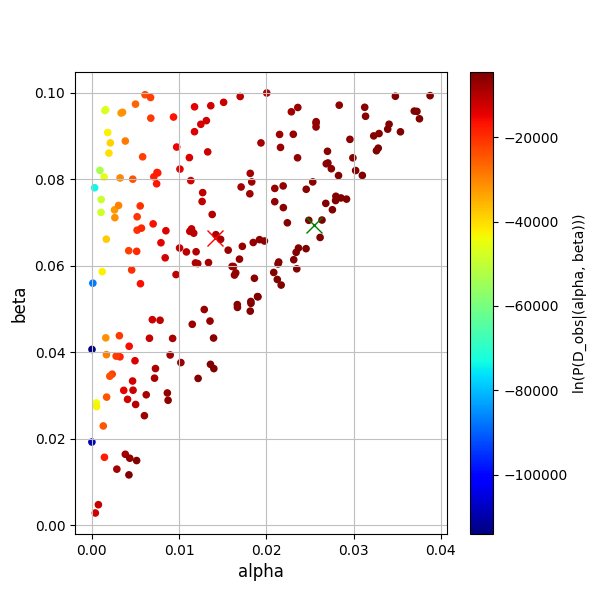
\includegraphics[width=\linewidth]{figures/sir1010_rfsmc.png}
        \caption{Sampled particles using Rational Functions SMC}
    \end{subfigure}
    \hfill
    \begin{subfigure}{0.48\textwidth}
        \centering
        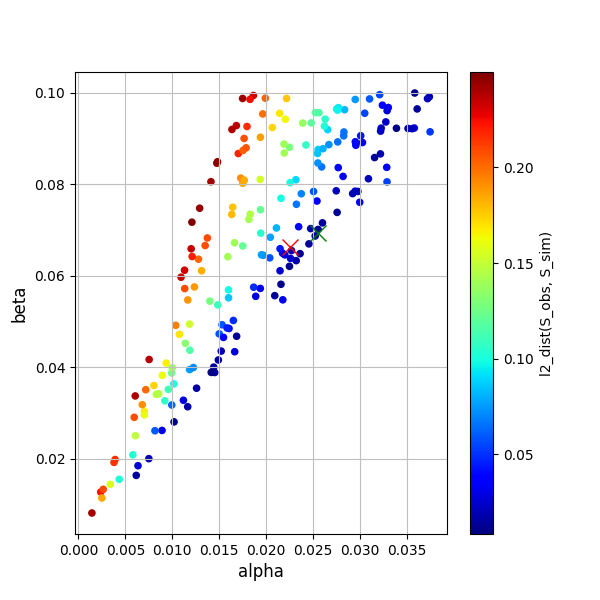
\includegraphics[width=\linewidth]{figures/sir1010_abcsmc.png}
        \caption{Sampled particles using Statiscal Model Checking ABC-SMC}
    \end{subfigure}
    \caption{SIR(10,1,0) parameter synthesis results.}
\end{figure}

In the experiment with $SIR(10,1,0)$ model we can see that  simulation based method deliver closer estimation to true parameter.

\begin{table}[H]
    \begin{tabular}{|l|c|l|}
        \hline
        \multicolumn{1}{|c|}{\textbf{SIR(15,1,0)}} & \multicolumn{1}{l|}{\begin{tabular}[c]{@{}l@{}}Rational function\\ SMC\end{tabular}}                                         & \begin{tabular}[c]{@{}l@{}}Statistical model checking\\ ABC-SMC\end{tabular} \\ \hline
        True parameter                             & \multicolumn{2}{c|}{(0.01724649, 0.06778604)}                                                                        \\ \hline
        Number of states                           & \multicolumn{2}{c|}{27}                                                                                              \\ \hline
        Number of BSCCs                            & \multicolumn{2}{c|}{6}                                                                                               \\ \hline
        Target property                            & \multicolumn{2}{c|}{$P_{\geq 0.25} [!(i>7) U^{<16} (i=0)]$}                                                          \\ \hline
        Synthetic data                             & \multicolumn{2}{c|}{(50,181,302,455,539,567,582,566,541,553,574,528,512,586,875,2589,)}                              \\ \hline
        Inferred parameter point                   & \multicolumn{1}{l|}{(0.02307652, 0.06481155)}                                           & (0.01758384, 0.06535699)   \\ \hline
        L2 distance to true parameter              & \multicolumn{1}{l|}{0.006544985909916083}                                               & 0.005519695496673707       \\ \hline
        Run time (hh:mm:ss)                        & \multicolumn{1}{l|}{1:07:36.442146}                                                     & 3:05:22.61795              \\ \hline
    \end{tabular}
    \caption{SIR(15,1,0) parameter estimation results.}
\end{table}

\begin{figure}[H]
    \centering
    \begin{subfigure}{0.48\textwidth}
        \centering
        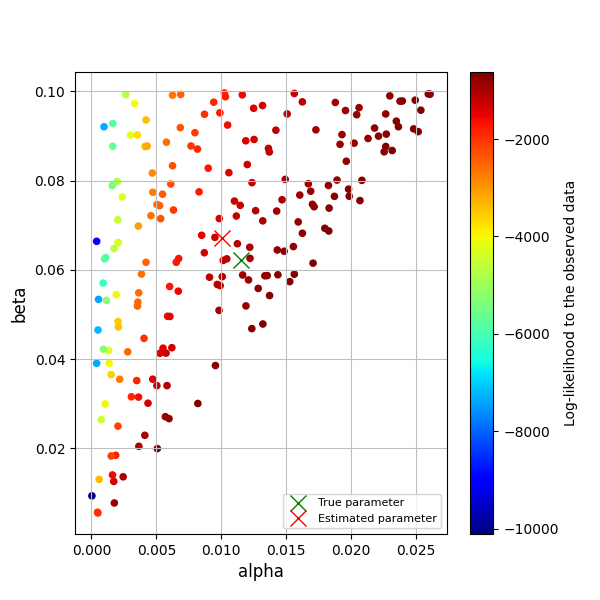
\includegraphics[width=\linewidth]{figures/sir1510_rfsmc.png}
        \caption{Sampled particles using Rational Functions SMC}
    \end{subfigure}
    \hfill
    \begin{subfigure}{0.48\textwidth}
        \centering
        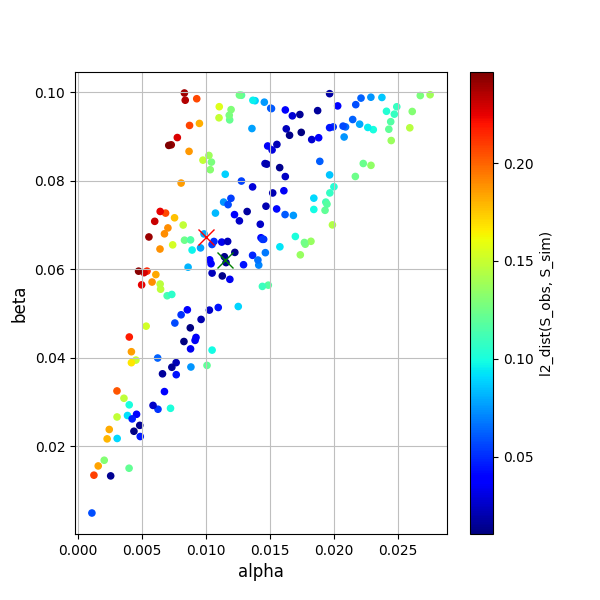
\includegraphics[width=\linewidth]{figures/sir1510_abcsmc.png}
        \caption{Sampled particles using Statiscal Model Checking ABC-SMC}
    \end{subfigure}
    \caption{SIR(15,1,0) parameter synthesis results.}
\end{figure}

\subsubsection{Parameter synthesis with uncertainty}
We introduce an uncertainty by merging BSCCs into 2 bins and use lower number of simulation to
generate synthetic data.
\begin{table}[H]
    \begin{tabular}{|l|c|l|}
        \hline
        \multicolumn{1}{|c|}{\textbf{SIR(15,1,0)}, BSCC merged} & \multicolumn{1}{l|}{\begin{tabular}[c]{@{}l@{}}Rational function\\ SMC\end{tabular}}             & \begin{tabular}[c]{@{}l@{}}Statistical model checking\\ ABC-SMC\end{tabular} \\ \hline
        True parameter                                          & \multicolumn{2}{c|}{(0.01724649, 0.06778604)}                                            \\ \hline
        Number of states                                        & \multicolumn{2}{c|}{27}                                                                  \\ \hline
        Number of BSCCs                                         & \multicolumn{2}{c|}{6}                                                                   \\ \hline
        Target property                                         & \multicolumn{2}{c|}{$P_{\geq 0.25} [!(i>7) U^{<16} (i=0)]$}                              \\ \hline
        Synthetic data                                          & \multicolumn{2}{c|}{(421,  834, 1126, 1362, 1851, 4406)}                                 \\ \hline
        Inferred parameter point                                & \multicolumn{1}{l|}{(0.02307652, 0.06481155)}               & (0.01758384, 0.06535699)   \\ \hline
        L2 distance to true parameter                           & \multicolumn{1}{l|}{0.006544985909916083}                   & 0.005519695496673707       \\ \hline
        Run time (hh:mm:ss)                                     & \multicolumn{1}{l|}{1:07:36.442146}                         & 3:05:22.61795              \\ \hline
    \end{tabular}
    \caption{SIR(5,1,0) parameter estimation results.}
\end{table}

\begin{figure}[H]
    \centering
    \begin{subfigure}{0.48\textwidth}
        \centering
        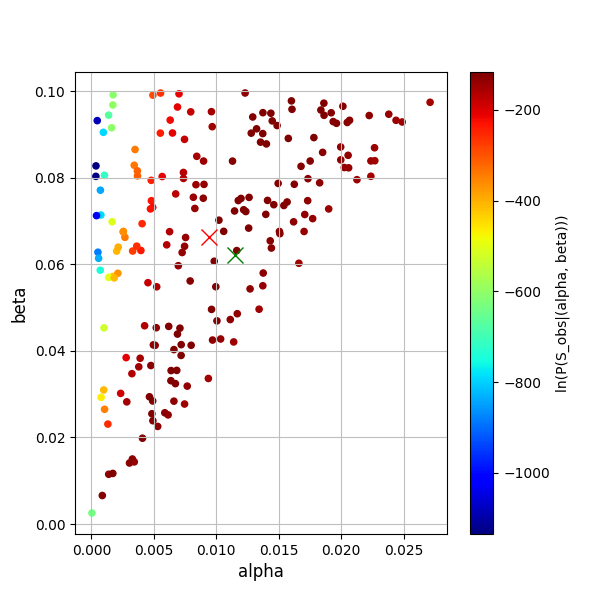
\includegraphics[width=\linewidth]{figures/sir1510_rfsmc_few.png}
        \caption{Sampled particles using Rational Functions SMC}
    \end{subfigure}
    \hfill
    \begin{subfigure}{0.48\textwidth}
        \centering
        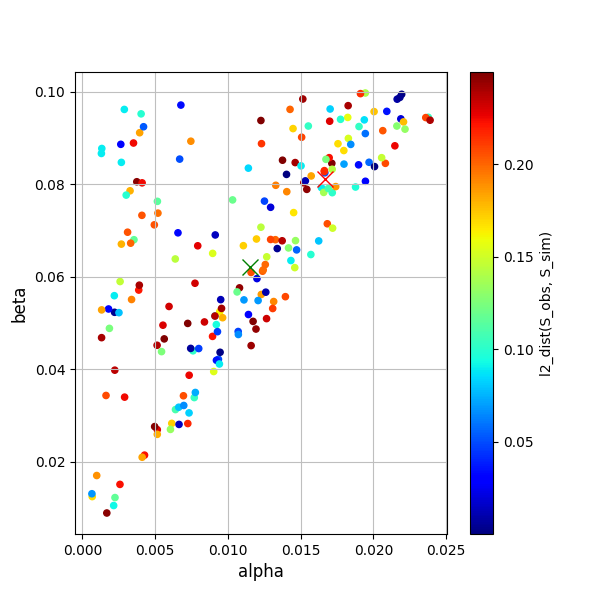
\includegraphics[width=\linewidth]{figures/sir1510_abcsmc_few.png}
        \caption{Sampled particles using Statiscal Model Checking ABC-SMC}
    \end{subfigure}
\end{figure}

\subsection{Discussion}
Unlike experiments with unmerged BSCCs, the experiment with merged BSCCs and simulation based
framework shows no general pattern of distance among satisfying parameter values.

